\section{Επίλυση πρωτεύοντος προβλήματος}

Η επίλυση του πρωτεύοντος προβλήματος απαιτεί την επίλυση της συνήθης διαφορικής εξίσωσης \ref{eq:primal} για την εύρεση της τιμής του πάχους του οριακού στρώματος κατά το μήκος της πλάκας. Έπειτα, απο την έκφραση \ref{eq:friction} υπολογίζουμε την τιμή της δύναμης της τριβής στην πλάκα λόγω του εισερχόμενου ρεύματος αέρα. 

\begin{equation}
    \Big(\dfrac{2}{\pi} - \dfrac{1}{2} \Big)\dfrac{U}{\nu}\delta(x)\dfrac{d\delta}{dx} + \dfrac{v_0(x)}{\nu}\delta(x) = \dfrac{\pi}{2} 
    \label{eq:primal}
\end{equation}



\begin{equation}
    \begin{aligned}
        F =& \int_0^L\tau_wdx \\[10pt]
        \tau_w =& \mu\dfrac{\partial u}{\partial y}\bigg|_{y=0}\\
    \end{aligned}
\label{eq:friction}
\end{equation}

όπου, 
\begin{itemize}
\item $\mathbf{\tau_w}$, είναι η διατμητική τάση στην επιφάνεια της πλάκας,
\item $\mathbf{u}$, είναι η τιμή της οριζόντιας ταχύτητας εντός του οριακού στρώματος
\end{itemize}

Μπορούμε να προσεγγίσουμε την κατανομή της οριζόντιας ταχύτητας ($u(y)$) με μια έκφραση που ικανοποιεί τις ακόλουθες συνθήκες:

$u(0) = 0$ και $u(\delta) = U$

Όπου $U$ είναι η ταχύτητα της ελεύθερης ροής.

Προσεγγίζοντας την κατανομή της ταχύτητας ως $u(y) = U\cdot \sin{\big(\dfrac{\pi}{2}\dfrac{y}{\delta}\big)}$, η διατμητική τάση στο επίπεδο της πλάκας εκφράζεται ως:

\begin{equation}
    \tau_w = \dfrac{U \pi \mu}{2 \delta (x)}
    \label{eq:shear}
\end{equation}

\begin{equation}
    F = \int_0^L \dfrac{U \pi \mu}{2 \delta (x)} dx
    \label{eq:finalFric}
\end{equation}

Η σ.δ.ε (εξίσωση \ref{eq:primal}) δεν έχει αναλυτική λύση. Έτσι, χρειάζεται να διακριτοποιήσουμε τη γεωμετρία (το μήκος) και να την επιλύσουμε αριθμητικά. Για την αριθμητική επίλυση χρησιμοποιήθηκε η μέθοδος Runge Kutta τέταρτης τάξης.

Αναδιαμορφώνουμε την εξίσωση \ref{eq:primal} και έχουμε
\begin{equation}
    f(x,\delta) = \dfrac{d\delta}{dx} =  \Big( \dfrac{\pi}{2} - \dfrac{v_0(x)}{\nu}\delta(x)\Big) \cdot \dfrac{1}{\big(\dfrac{\pi}{2}-\dfrac{1}{2}\big)\dfrac{U}{\nu}\delta(x)}
\label{eq:rungePrimal}
\end{equation}

Και το σχήμα της Runge Kutta υλοποιείται ως εξής:

\begin{equation}
    \begin{aligned}
        k_1 =& \Delta x f\big(x^i, \delta^i\big)\\[3pt]
        k_2 =& \Delta x f\Big(x^i + \dfrac{\Delta x}{2}, \delta^i + \dfrac{k_1}{2}\Big)\\[3pt]
        k_3 =& \Delta x f\Big(x^i + \dfrac{\Delta x}{2}, \delta^i + \dfrac{k_2}{2}\Big)\\[5pt]
        k_4 =& \Delta x f\big(x^{i+1} , \delta^i + k_3\big)\\[12pt]
        \delta^{i+1} =& \delta^i + \dfrac{1}{6}\big(k_1+k_2+k_3+k_4\big)
    \end{aligned}
\end{equation}

Επομένως, λαμβάνουμε έτσι τις κομβικές τιμές για το πάχος του οριακού στρώματος, και έτσι, μπορούμε να ολοκληρώσουμε αριθμητικά (με τη μέθοδο των τραπεζίων) την σχέση \ref{eq:finalFric} και να λάβουμε την τιμή της αντικειμενικής συνάρτησης (της τριβής).

\begin{equation}
    F = \sum_{i=0}^{N-1}\Bigg[\Big(\dfrac{U\pi\mu}{2\delta_i}+\dfrac{U\pi\mu}{2\delta_{i+1}}\Big)\dfrac{x_{i+1}-x_i}{2}\Bigg]
\label{eq:trapzFric}
\end{equation}

\subsection{Υλοποίηση υπολογισμών και αποτελέσματα}

Για την ολοκλήρωση της εξίσωσης \ref{eq:primal} απαιτείται μια οριακή συνθήκη. Για οριακή συνθήκη ορίζουμε το πάχος του οριακού στρώματος στην αρχή της πλάκας ($x=0$) να είναι μηδενικό ($\delta(0)=0$). Ωστόσο, όπως υποδεικνύεται και απο την εκφώνηση και όπως παρατηρείται και απο την έκφραση της \ref{eq:rungePrimal}, μια μηδενική τιμή απειρείζει η τιμή της παραγώγου, έτσι σε μια αριθμητική μέθοδο δεν μπορεί να βοηθήσει για την εξέλιξη των υπολογισμών. Έτσι, ορίζουμε μια μικρή τιμή, της τάξης των $(10^{-6}-10^{-3})$ ώστε να μην επηρεάσει τα αποτελέσματά μας, αλλά να επιτρέπει την επίλυση της σ.δ.ε. 

Σημειώνεται πως έγινε δοκιμή για τοπική πύκνωση στους κόμβους στην αρχή (ή και στο τέλος) της πλάκας και βοήθησε στα αποτελέσματα για ίδιο αριθμό κόμβων, ωστόσο, στη συνέχεια της εργασίας, στον υπολογισμό των του συζυγούς πεδίου με τη συνεχή μέθοδο, έβλαψε τα αποτελέσματά της μεθόδου. Έτσι, υιοθετήσαμε μια μεγαλύτερη τιμή ίση με $\delta(0) = 10^{-3}$, και ομοιόμορφο πλέγμα.

\subsubsection{Ανάλυση ανεξαρτησίας κομβικών σημείων}

Για τον καθορισμό του αριθμού των κομβικών σημείων που οδηγούν σε ικανοποιητικά αποτελέσματα της αντικειμενικής συνάρτησης, έγινε ανάλυση ανεξαρτησίας της τριβής ως προς τον αριθμό των κομβικών σημείων. Συγκεκριμένα, έγινε δοκιμή στο εύρος ($100-2000$) σημείων, με ομοιόμορφη απόσταση. Τα αποτελέσματα παρατίθενται στο σχήμα \ref{fig:node_Friction}.


\begin{figure}[h!]
    \centering
    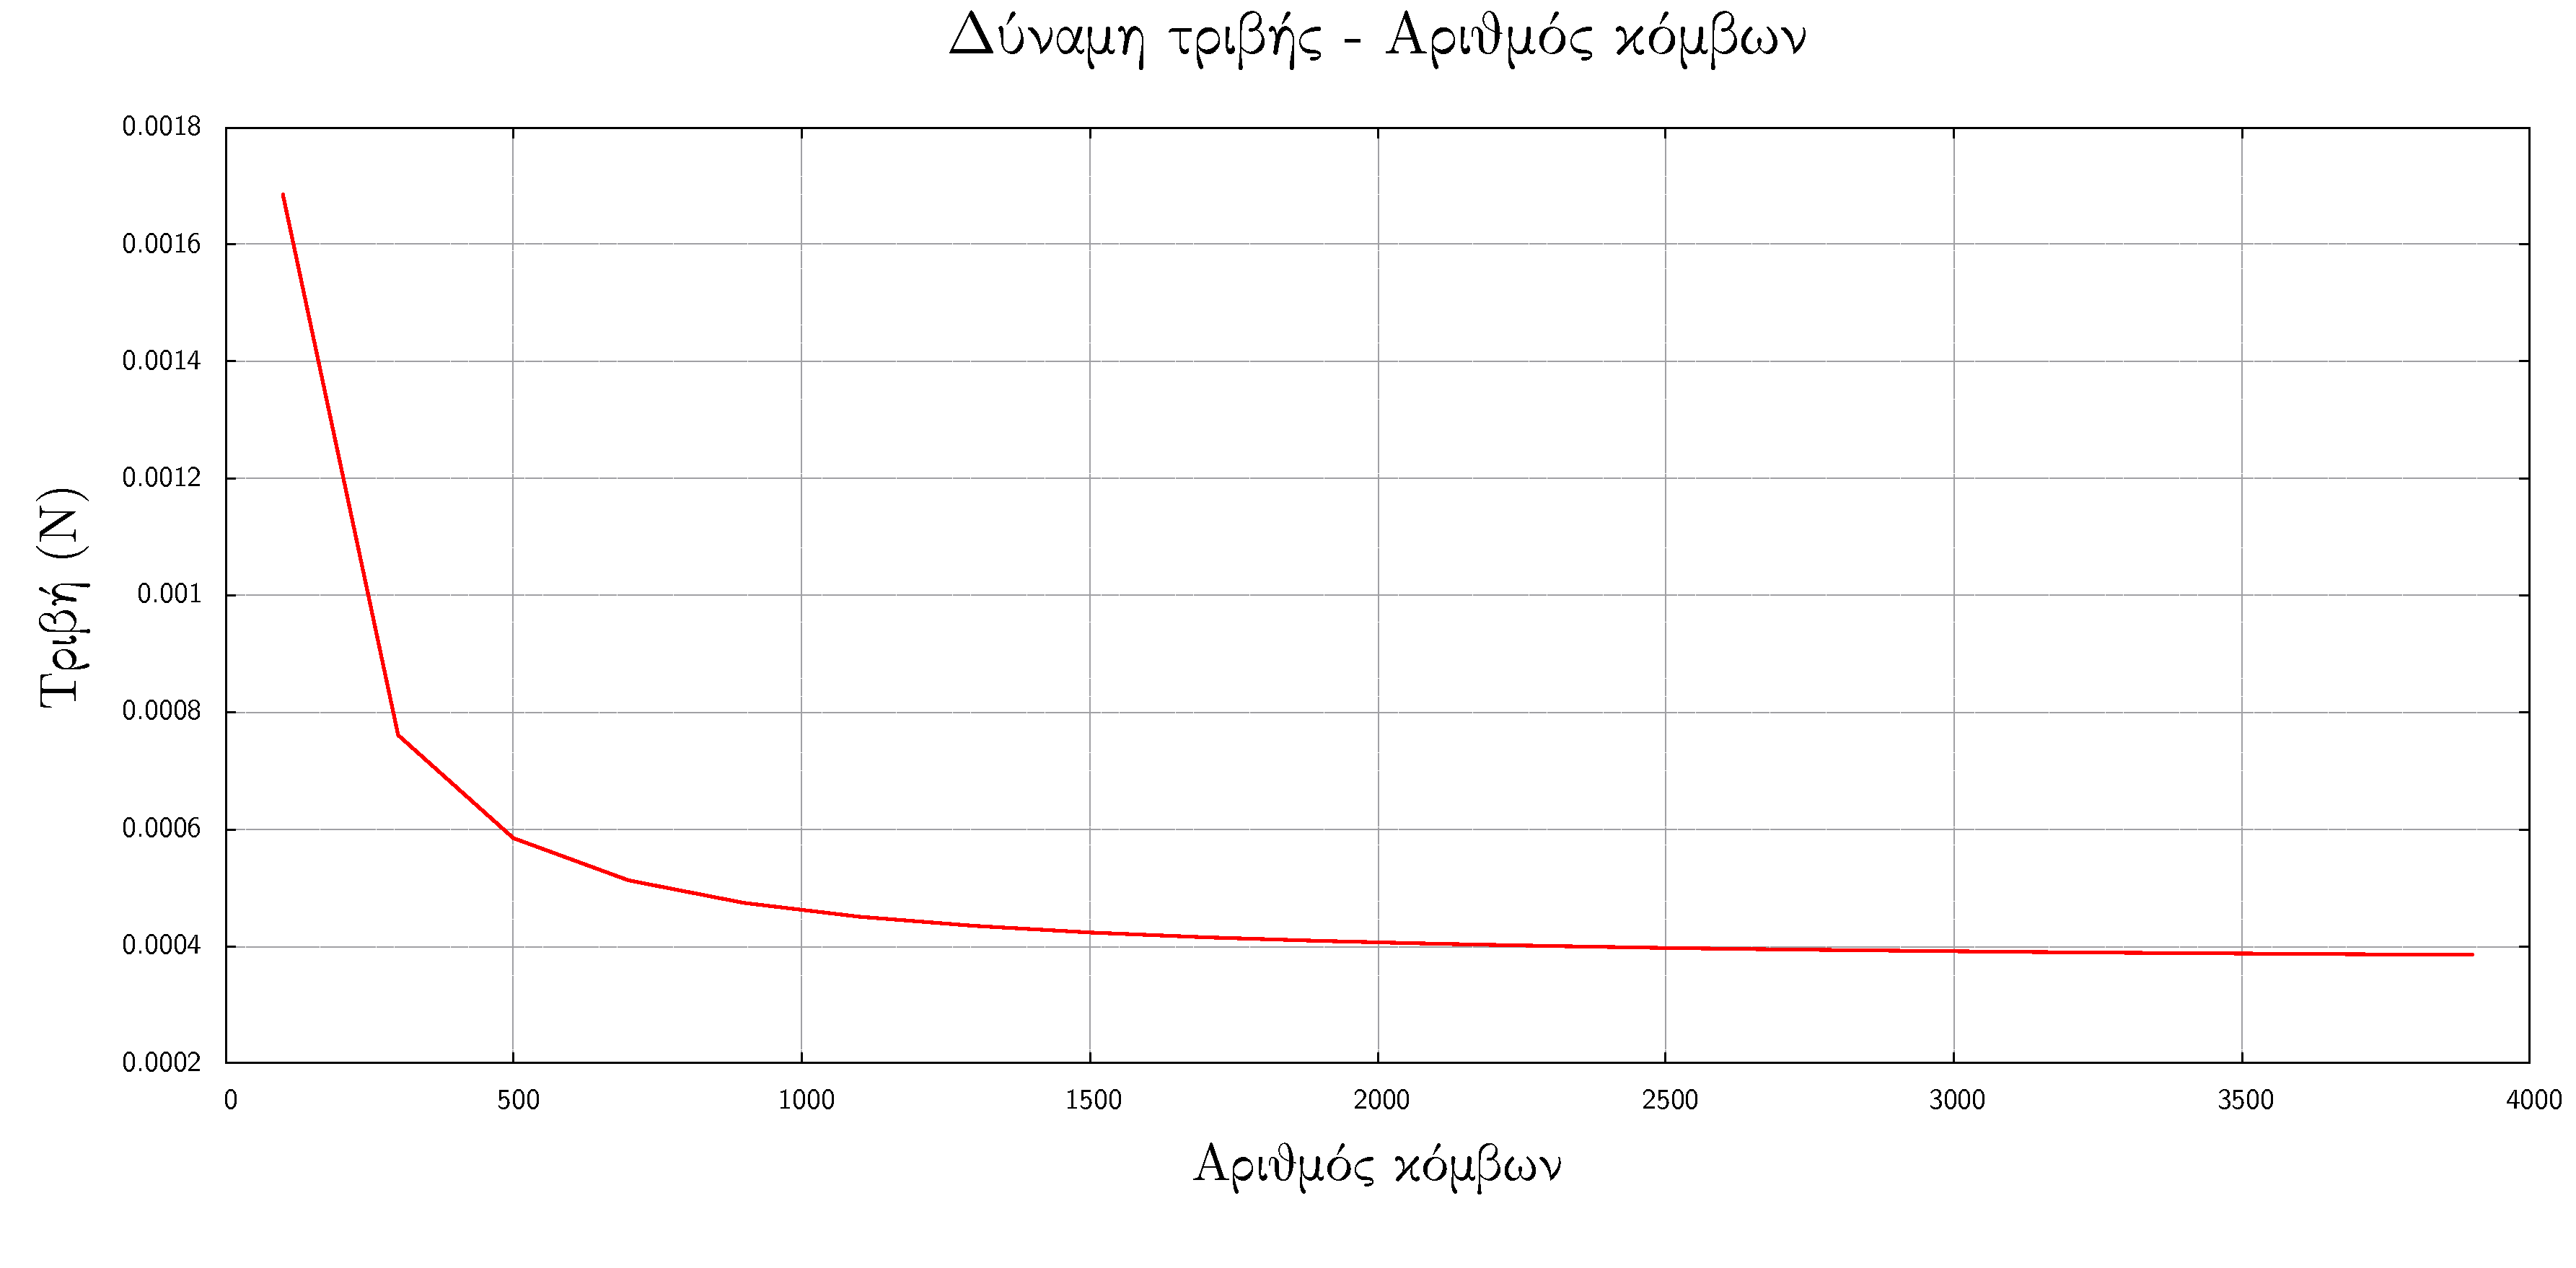
\includegraphics[width=.85\textwidth]{figures/node_dep.pdf}
    \caption{Δύναμη τριβής συναρτήσει του αριθμού των κόμβων}
    \label{fig:node_Friction}
\end{figure}

Όπως φαίνεται και στο σχήμα \ref{fig:node_Friction}, η τιμή της αντικειμενικής συνάρτησης αρχίζει να σταθεροποιείται περίπου στους 2000 κόμβους, επομένως, συνεχίζοντας, όλα τα μοντέλα θα έχουν τον ίδιο αριθμό κόμβων.

Παρακάτω, στο σχήμα \ref{fig:velProf} παρατίθεται το διάγραμμα της μεταβολής του πάχους του οριακού στρώματος ($\delta(x)$) κατά το μήκος της πλάκας καθώς και το προφίλ της ταχύτητας εντός του οριακού στρώματος στο κέντρο της πλάκας ($x=L/2$).

\begin{figure}[h!]
    \centering
    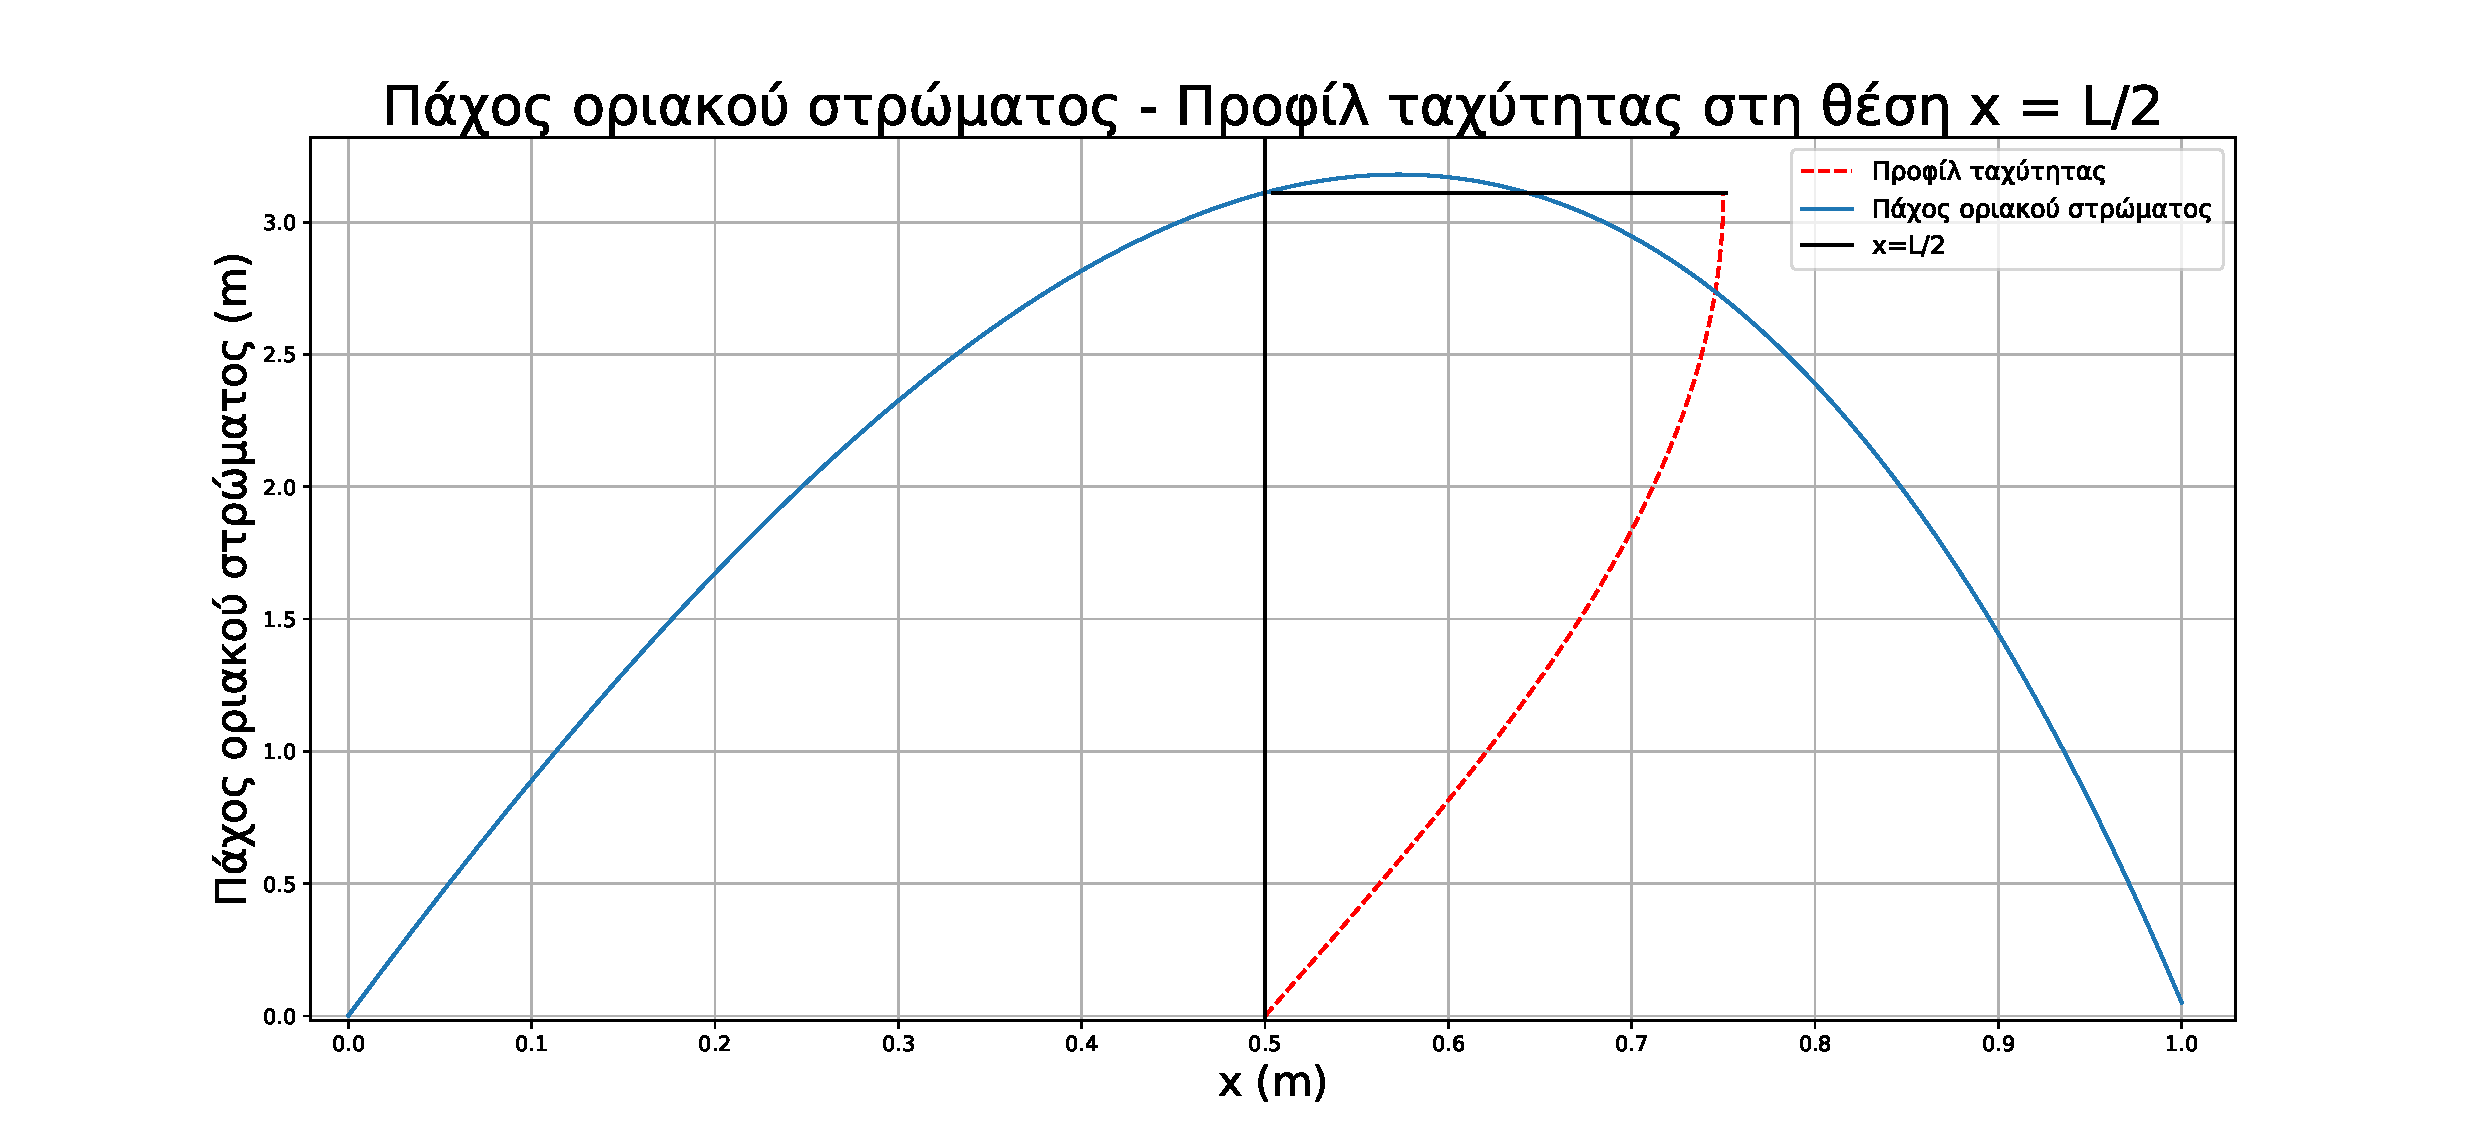
\includegraphics[width=.85\textwidth]{figures/velocity_profile.pdf}
    \caption{Πάχος οριακού στρώματος και προφίλ ταχύτητας στη μέση της πλάκας}
    \label{fig:velProf}
\end{figure}

